\documentclass[useAMS,usenatbib,a4paper]{mn2e}

\pdfpagewidth=\paperwidth 
\pdfpageheight=\paperheight

\newcommand{\sub}[2]{\ensuremath{#1_{\mathrm{#2}}}}
\newcommand{\super}[2]{\ensuremath{#1^{\mathrm{#2}}}}
\newcommand{\rcore}{\sub{r}{core}}
\newcommand{\unit}[2]{\ensuremath{\textrm{#1}^{#2}}}
\newcommand{\half}{\frac{1}{2}}
%\newcommand\aj{{AJ}}% 
          % Astronomical Journal 
\newcommand\araa{{ARA\&A}}% 
          % Annual Review of Astron and Astrophys 
\newcommand\apj{{ApJ}}% 
          % Astrophysical Journal 
\newcommand\apjl{{ApJ}}% 
          % Astrophysical Journal, Letters 
\newcommand\apjs{{ApJS}}% 
          % Astrophysical Journal, Supplement 
\newcommand\ao{{Appl.~Opt.}}% 
          % Applied Optics 
\newcommand\apss{{Ap\&SS}}% 
          % Astrophysics and Space Science 
\newcommand\aap{{A\&A}}% 
          % Astronomy and Astrophysics 
\newcommand\aapr{{A\&A~Rev.}}% 
          % Astronomy and Astrophysics Reviews 
\newcommand\aaps{{A\&AS}}% 
          % Astronomy and Astrophysics, Supplement 
\newcommand\azh{{AZh}}% 
          % Astronomicheskii Zhurnal 
\newcommand\baas{{BAAS}}% 
          % Bulletin of the AAS 
\newcommand{\jcap}{J. Cosm. Astropart. Phys.}
	% Journal of Cosmology and Astroparticle Physics
\newcommand\jrasc{{JRASC}}% 
          % Journal of the RAS of Canada 
\newcommand\memras{{MmRAS}}% 
          % Memoirs of the RAS 
\newcommand\mnras{{MNRAS}}% 
          % Monthly Notices of the RAS 
\newcommand\pra{{Phys.~Rev.~A}}% 
          % Physical Review A: General Physics 
\newcommand\prb{{Phys.~Rev.~B}}% 
          % Physical Review B: Solid State 
\newcommand\prc{{Phys.~Rev.~C}}% 
          % Physical Review C 
\newcommand\prd{{Phys.~Rev.~D}}% 
          % Physical Review D 
\newcommand\pre{{Phys.~Rev.~E}}% 
          % Physical Review E 
\newcommand\prl{{Phys.~Rev.~Lett.}}% 
          % Physical Review Letters 
\newcommand\pasp{{PASP}}% 
          % Publications of the ASP 
\newcommand\pasj{{PASJ}}% 
          % Publications of the ASJ 
\newcommand\qjras{{QJRAS}}% 
          % Quarterly Journal of the RAS 
\newcommand\skytel{{S\&T}}% 
          % Sky and Telescope 
\newcommand\solphys{{Sol.~Phys.}}% 
          % Solar Physics 
\newcommand\sovast{{Soviet~Ast.}}% 
          % Soviet Astronomy 
\newcommand\ssr{{Space~Sci.~Rev.}}% 
          % Space Science Reviews 
\newcommand\zap{{ZAp}}% 
          % Zeitschrift fuer Astrophysik 
\newcommand\nat{{Nature}}% 
          % Nature 
\newcommand\iaucirc{{IAU~Circ.}}% 
          % IAU Cirulars 
\newcommand\aplett{{Astrophys.~Lett.}}% 
          % Astrophysics Letters 
\newcommand\apspr{{Astrophys.~Space~Phys.~Res.}}% 
          % Astrophysics Space Physics Research 
\newcommand\bain{{Bull.~Astron.~Inst.~Netherlands}}% 
          % Bulletin Astronomical Institute of the Netherlands 
\newcommand\fcp{{Fund.~Cosmic~Phys.}}% 
          % Fundamental Cosmic Physics 
\newcommand\gca{{Geochim.~Cosmochim.~Acta}}% 
          % Geochimica Cosmochimica Acta 
\newcommand\grl{{Geophys.~Res.~Lett.}}% 
          % Geophysics Research Letters 
\newcommand\jcp{{J.~Chem.~Phys.}}% 
          % Journal of Chemical Physics 
\newcommand\jgr{{J.~Geophys.~Res.}}% 
          % Journal of Geophysics Research 
\newcommand\jqsrt{{J.~Quant.~Spec.~Radiat.~Transf.}}% 
          % Journal of Quantitiative Spectroscopy and Radiative Trasfer 
\newcommand\memsai{{Mem.~Soc.~Astron.~Italiana}}% 
          % Mem. Societa Astronomica Italiana 
\newcommand\nphysa{{Nucl.~Phys.~A}}% 
          % Nuclear Physics A 
\newcommand\physrep{{Phys.~Rep.}}% 
          % Physics Reports 
\newcommand\physscr{{Phys.~Scr}}% 
          % Physica Scripta 
\newcommand\planss{{Planet.~Space~Sci.}}% 
          % Planetary Space Science 
\newcommand\procspie{{Proc.~SPIE}}% 
          % Proceedings of the SPIE 
\let\astap=\aap 
\let\apjlett=\apjl 
\let\apjsupp=\apjs 
\let\applopt=\ao 


\bibliographystyle{astron}

\usepackage{graphicx} 
\usepackage{epstopdf} 
\usepackage{amsmath}
\usepackage{hyperref}

\begin{document}

\title{Action-space clustering of tidal streams can be used to map the Galactic potential}
%authors in no particular order
\author[]{Robyn E. Sanderson, Amina Helmi${}^{1}$, David Hogg${}^{2}$\\
${}^{1}$Kapteyn Astronomical Institute, P.O. Box 800, 9700 AV Groningen, The Netherlands\\
${}^{2}$NYU}

\maketitle

\begin{abstract}
We use a simple example to demonstrate that, given a parameterized model of the Galactic potential, the set of parameters retrieved by maximizing the Kullback-Leibler divergence of a set of stars initially clustered in action space (e.g. stars in tidal streams) are the input parameters. This method will allow us to capitalize on the existence of kinematic substructures in the Galaxy to map its gravitational potential. Adding more streams improves the constraints on the best-fit parameters by breaking degeneracies between parameters; adding more stars to existing streams improves the tightness of the constraints. We also demonstrate that Gaia will measure the phase-space positions of red giant stars with sufficient accuracy to use this technique, and that ground-based spectroscopic follow-up to obtain radial velocities of faint halo stars offers substantial improvement over results obtained with Gaia data alone. 
\end{abstract}

%\begin{keywords}
%\end{keywords}

\section{Introduction}
\label{sec:intro}

\section{The Kullback-Liebler divergence}
\label{sec:kld}

The Kullback-Liebler divergence (KLD) is a way of comparing the degree of clustering (or amount of information) in two different statistical distributions. For a continuous random variable $\mathbf{x}$, the KLD \emph{from} distribution $p(\mathbf{x})$ \emph{to} distribution $q(\mathbf{x})$ is defined as
\begin{equation}
 D_{KL}(p\to q) \equiv \int p(\mathbf{x}) \log \frac{p(\mathbf{x})}{q(\mathbf{x})} d\mathbf{x}.
\end{equation}
The KLD is not symmetric; it can be considered a measure of the relative entropy between $p$ and $q$. The lower the entropy of $p$ relative to $q$, the higher the value of $D_{KL}$ (Figure \ref{fig:1Dexample}).
\begin{figure*}
 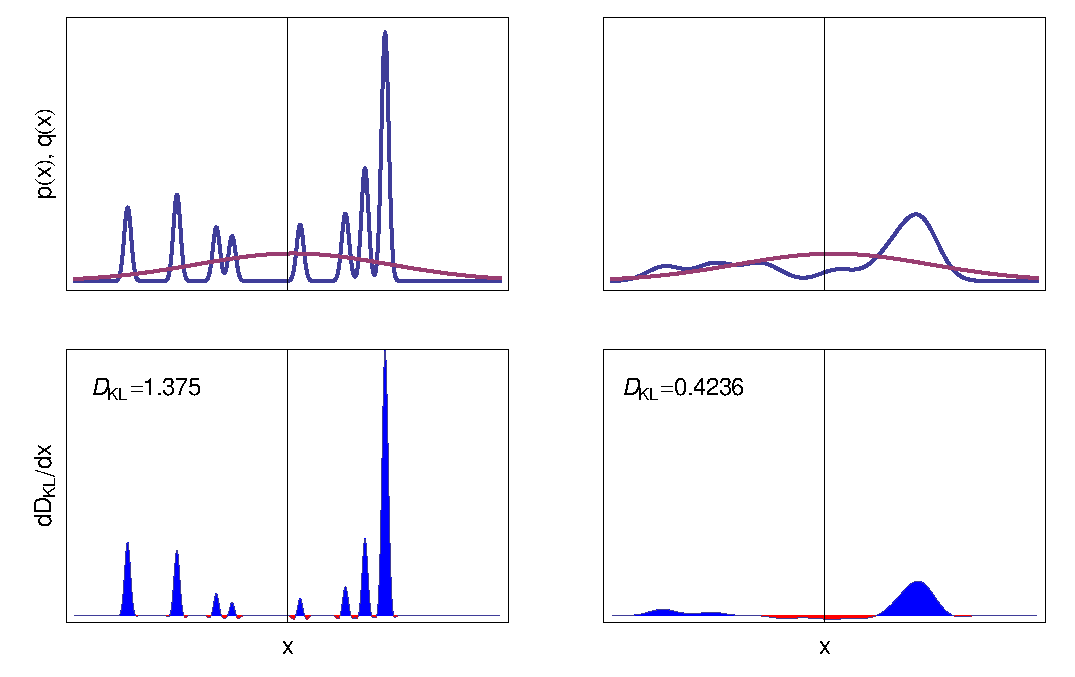
\includegraphics[width=0.95\textwidth]{KLDiv_1D_Example}
\caption{If the distribution $p$ (blue line) is much more clustered than distribution $q$ (pink line) as shown in the example on the left (upper panel), then the integrand (lower panel) is large and $D_{KL}$ is large. A distribution $p$ that is only somewhat less smooth than $q$ (right column) has a lower $D_{KL}$.}
\label{fig:1Dexample}
\end{figure*}

If a set of $N$ points $\mathbf{x}_i$ are independent random deviates drawn from $p$, then we can use them to do a Monte Carlo approximation to the integral:
\begin{equation}
  \tilde{D}_{KL}(p\to q) = \frac{1}{N} \sum_{i}^{N} \log \frac{p(\mathbf{x}_i)}{q(\mathbf{x}_i)}
\end{equation}
This works even if $p$ is not known. In that case you use the ``observed'' distribution $\tilde{p}$ constructed in some way (e.g. using a density estimator) from the observed $\mathbf{x}_i$ instead of the true distribution $p$. 

% An example using the two distributions on the left of Figure \ref{fig:1Dexample} is shown in Figure \ref{fig:monteCarlo}.
% \begin{figure*}
%  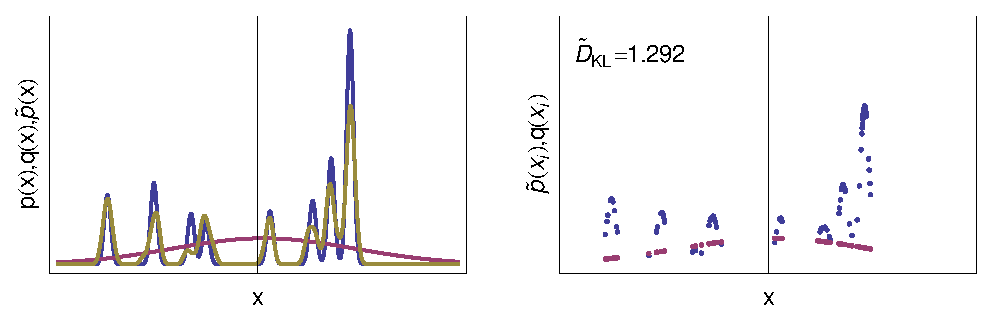
\includegraphics[width=0.95\textwidth]{monteCarlo}
% \caption{Left panel: The observed distribution $\tilde{p}$ (yellow) can be constructed from the $\mathbf{x}_i$ (in this case using Gaussian smoothing) to approximate the true parent distribution $p$ (blue). Right panel: Both $\tilde{p}$ (blue) and $q$ (pink) are evaluated at the $\mathbf{x}_i$ to calculate the estimated KLD, $\tilde{D}_{KL}$. The value obtained is close to the one found using the exact parent distribution.}
% \label{fig:monteCarlo}
% \end{figure*}

Finally, since $p$ and $q$ are probability distributions, the KLD is invariant under transformations of $\mathbf{x}$ because $p(\mathbf{x}) d\mathbf{x} = p(\mathbf{y}) d\mathbf{y}$, for any continuously differentiable $\mathbf{y}(\mathbf{x})$:
\begin{eqnarray}
  \int  \log \frac{p(\mathbf{x})}{q(\mathbf{x})} p(\mathbf{x}) d\mathbf{x} &=& \int \log \frac{p(\mathbf{y}) d\mathbf{y}/d\mathbf{x}}{q(\mathbf{y})d\mathbf{y}/d\mathbf{x}} p(\mathbf{y}) d\mathbf{y} \nonumber \\
  &=&  \int  \log \frac{p(\mathbf{y})}{q(\mathbf{y})} p(\mathbf{y}) d\mathbf{y} 
\end{eqnarray}


The KLD is a promising tool for using stellar streams to constrain the Galactic potential because stream stars should be clustered in action space. The clustering of streams in action space is assumed to be tightest when the correct potential (or the closest one to the real potential) is used to compute the actions from the coordinates $(\mathbf{x},\mathbf{v})$. So if we take the actions $\mathbf{I}$ as the random variable, we can compare the observed distribution $\tilde{O}(\mathbf{I}|\mathbf{a})$ obtained by computing the values $\mathbf{I}_i$ for a given set of potential parameters $\mathbf{a}$ to a smooth distribution $\tilde{T}$ that fits the same actions using the Monte-Carlo form $\tilde{D}_{KL}$:
\begin{equation}
\label{eq:KLD_perfect}
\sub{\tilde{D}}{KL} \equiv \sum_i^{N_*} \log \frac{\tilde{O}[\mathbf{I}_i(\mathbf{a})|\mathbf{a}]}{\tilde{T}[\mathbf{I}_i(\mathbf{a})|\mathbf{a}]}
\end{equation}
The tildes are intended to distinguish the distributions $\tilde{O}$ and $\tilde{T}$ that are inferred from the discrete set of $\mathbf{I}_i$ from the true underlying continuous distributions $O$ and $T$, from which these $\mathbf{I}_i$ are drawn.

As the parameters approach the best-fit potential, the value of $\tilde{D}_{KL}$ will increase as the actions of stars in the various streams cluster more tightly together. Figure \ref{fig:actionClustering} shows a simple example using the radial action of the isochrone potential, a simple two-parameter potential for which the actions have analytic expressions. Changing either of the parameters away from the input value produces a broader distribution and hence a smaller $\tilde{D}_{KL}$. In this example, the enclosed-mass degeneracy is also evident, since the distribution varies in opposite directions for a change of the same sign in $M$ or $b$. This means that raising $M$ can be compensated by lowering $b$, and vice versa. The means to break this degeneracy is also evident: streams centered around different values of $J_r$ have distributions that respond differently to changes in $M$ and $b$, especially at large $J_r$ (more radial orbits). Adding more streams probes a larger range of orbits and breaks the enclosed-mass degeneracy.
\begin{figure*}
 \begin{tabular}{cc}
 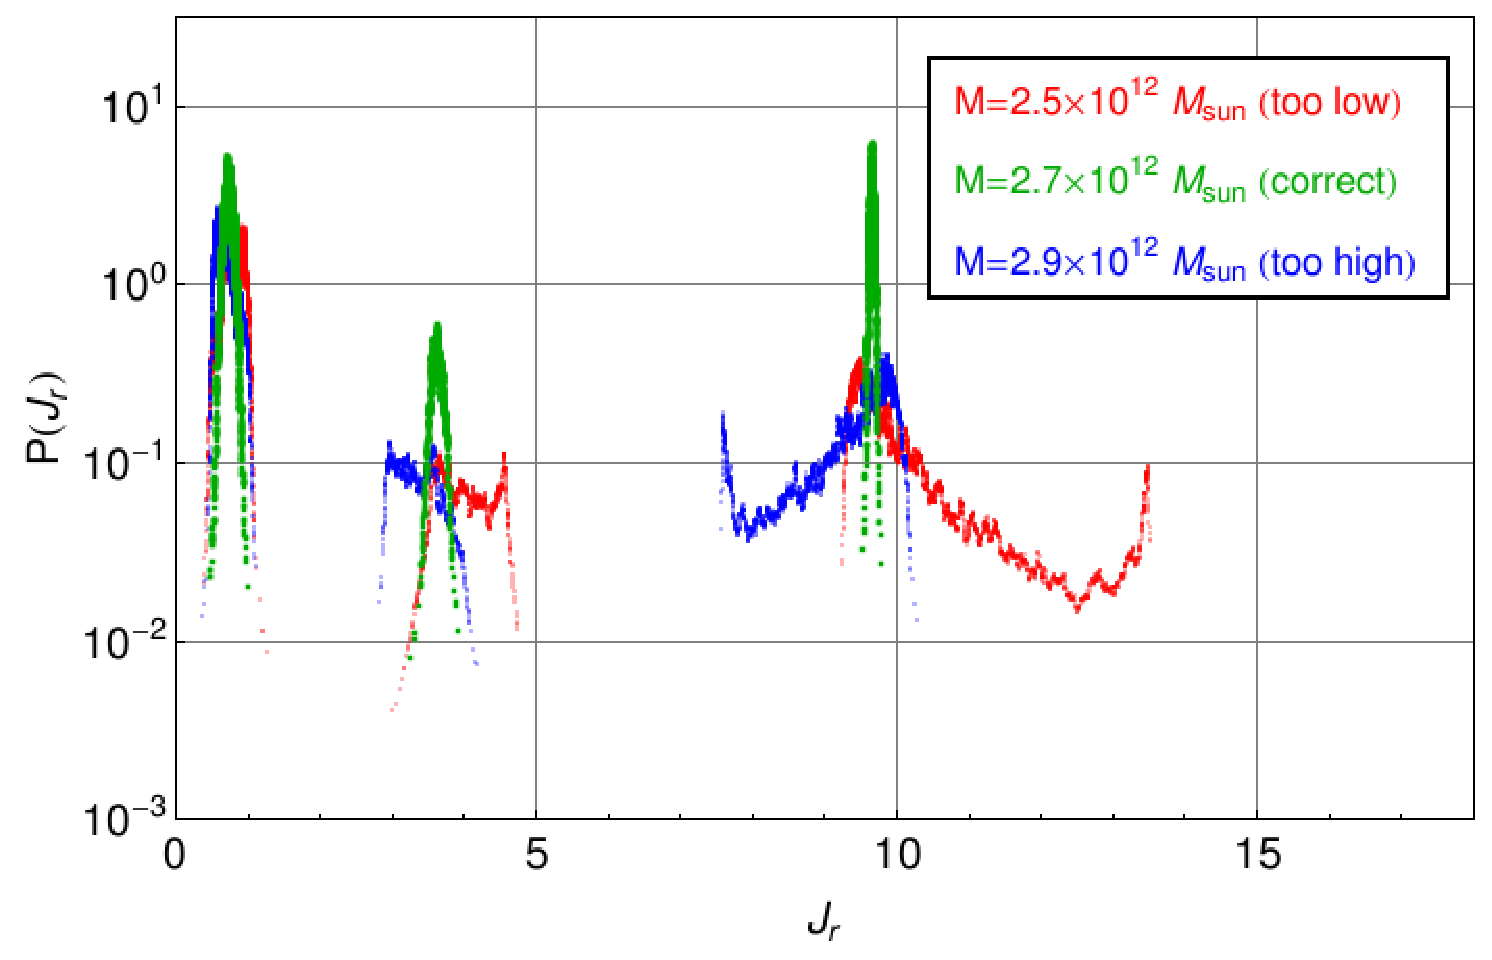
\includegraphics[width=0.45\textwidth]{ActionClusteringFigureMass} & 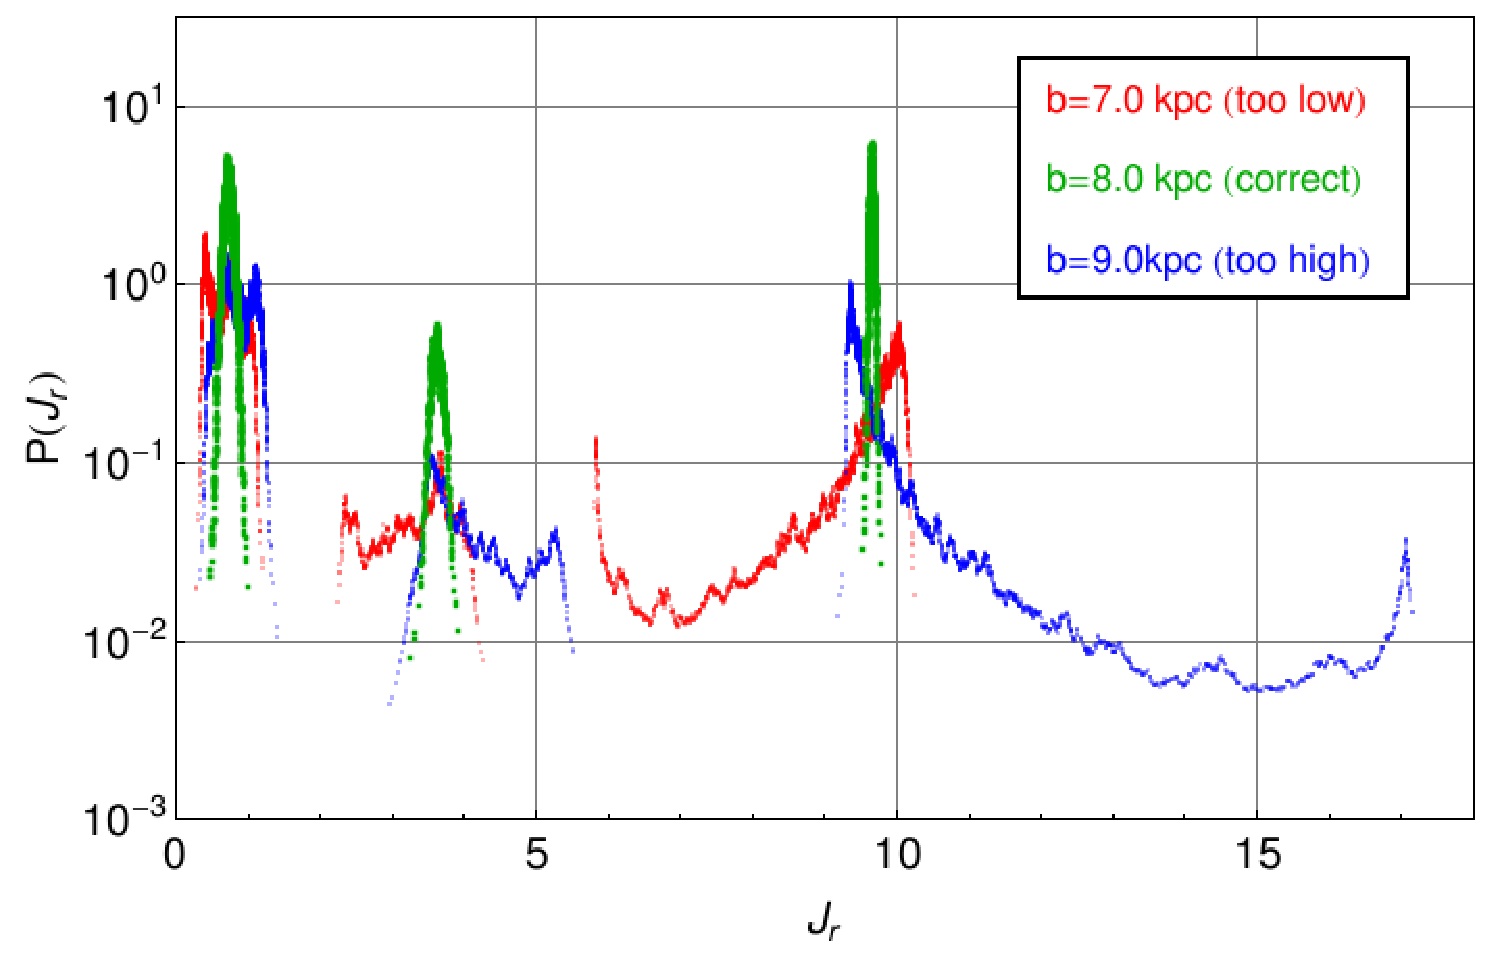
\includegraphics[width=0.45\textwidth]{ActionClusteringFigureRadius}
\end{tabular}
\caption{Given coordinates $\mathbf{x},\mathbf{p})$ for a set of stream stars, the distribution of calculated radial actions $J_r$ is most clustered when the potential parameters (in this case the scale mass $M$ and scale radius $b$) are equal to the input values. This example uses three streams with a total of 50,000 ``stars''; the distribution $P(J_r)$ is computed by a one-dimensional nearest-neighbor density estimator with $n_{NN}=50$.}
\label{fig:actionClustering}
\end{figure*}


% The KLD is invariant under parameter transformations, but we've also collapsed it to 3D from 6D by only considering the actions. So somehow we have to account for $\mathbf{a}$-dependence if we try to transform back to observables. We can define the 6D distributions $p$ and $q$ by giving them both the same $\mathbf{\Theta}$-dependence:
% \begin{equation}
%  p(\mathbf{I},\mathbf{\Theta}) = p(\mathbf{I})f(\mathbf{\Theta}), \qquad  q(\mathbf{I},\mathbf{\Theta}) = q(\mathbf{I})f(\mathbf{\Theta})
% \end{equation} 
% so that 
% \begin{equation}
%  p(\mathbf{I}) = \int d\mathbf{\Theta}\ p(\mathbf{I})f(\mathbf{\Theta}) \qquad \textrm{and} \qquad \frac{p(\mathbf{I},\mathbf{\Theta})}{q(\mathbf{I},\mathbf{\Theta})} = \frac{p(\mathbf{I})f(\mathbf{\Theta})}{q(\mathbf{I})f(\mathbf{\Theta})} = \frac{ p(\mathbf{I})}{q(\mathbf{I})}
% \end{equation} 
% Then if we are working with the continuous distributions we get that
% \begin{equation}
%  D_{KL} = \int p(\mathbf{I}) \log \frac{p(\mathbf{I})}{q(\mathbf{I})} d\mathbf{I} = \int p(\mathbf{I},\mathbf{\Theta}) \log \frac{p(\mathbf{I},\mathbf{\Theta})}{q(\mathbf{I},\mathbf{\Theta})} d\mathbf{I}\ d\mathbf{\Theta}.
% \end{equation} 
% It appears that then if we transform back to observables $\mathbf{w}(\mathbf{I},\mathbf{\Theta})$, then we should get the same result for $D_{KL}$. However we also know that $p$ and $q$ depend on the parameters $\mathbf{a}$ of the potential so we really should write
% \begin{equation}
%   D_{KL} =\int p(\mathbf{I},\mathbf{\Theta}|\mathbf{a}) \log \frac{p(\mathbf{I},\mathbf{\Theta}|\mathbf{a})}{q(\mathbf{I},\mathbf{\Theta}|\mathbf{a})} d\mathbf{I}\ d\mathbf{\Theta}
% \end{equation} 
% So we are still only working with conditional probabilities. I am not sure how to make the parameter transformation in this case; I suspect if we do it right there will be a Hessian that appears, dependent on the parameters, even in the observable case. Not sure where this goes quite yet.


\section{Process}
\label{sec:process}

We can use a simple example to test whether the KL-divergence can be used to recover input values for streams in a gravitational potential. In this section we describe the steps in this process. 

\subsection{Potential and input parameters}
First we choose a potential parameterization and a set of input parameters $\sub{\mathbf{a}}{true}$. For our example we choose the isochrone potential
\begin{equation}
 \Phi(r) = -\frac{M}{b+\sqrt{r^2+b^2}}
\end{equation} 
 because it has analytic expresssions for the actions $(J_r,L)$, where $L$ is the absolute value of the total angular momentum and $J_r$ is the radial action
\begin{equation}
 J_r = \frac{G M}{\sqrt{-2E}} - \half \left(L+\sqrt{L^2 + 4 G M b}\right).
\end{equation}
The specific energy $E$ is given by the standard expression
\begin{equation}
 E = \half \mathbf{v}\cdot\mathbf{v} + \Phi(r).
\end{equation} 
The isochrone potential is actually not a very good match to what we know about the shape of the real Milky Way or about simulated cosmological dark matter halos. In particular, this potential is spherically symmetric, whereas the degree of flattening of the Galactic potential is actually of great interest. In principle any parameterization for which the actions can be calculated will work; for simplicity we start with an analytically tractable example.

\subsection{Making the streams}
To make the streams with which the potential is to be constrained, we construct a distribution of actions $\sub{\mathbf{I}}{true}(\mathbf{I})$ that models a set of $N_s$ streams $\mathbf{I}_s(\mathbf{I})$.
\begin{equation}
 \sub{\mathbf{I}}{true}(\mathbf{I}) = \sum_s^{N_s} p_s \mathbf{I}_s(\mathbf{I}), \qquad \sum_s^{N_s} p_s = 1
\end{equation} 
%Later on we can also add a smooth background $\mathbf{I}_b(\mathbf{I})$, to test the sensitivity of the method to interloper stars that have been misidentified as stream members:
%\begin{equation}
% \sub{\mathbf{I}}{true}(\mathbf{I}) = \sum_s^{N_s} p_s \mathbf{I}_s(\mathbf{I}) + (1-\sum_s^{N_s} p_s) \mathbf{I}_b(\mathbf{I}), \qquad \sum_s^{N_s} p_s < 1
%\end{equation} 
The probabilities $p_s$ that stars are in a particular stream can be used to explore the effect of different stellar masses in the progenitor satellites. 

We reperesent each stream as a multivariate Gaussian at a locations $\mathbf{I}_{0,s}$ in action space, with covariance matrix $\mathbf{\sigma}_s$ in $k$ dimensions ($k=2$ for a spherical potential and 3 otherwise): 
\begin{equation}
 \mathbf{I}_s = \frac{1}{\sqrt{(2 \pi)^k \det \mathbf{\sigma}_s}} e^{-(\mathbf{I}-\mathbf{I}_{0,s})^T \mathbf{\sigma}_s^{-1} (\mathbf{I}-\mathbf{I}_{0,s})/2}
\end{equation} 
The location $\mathbf{I}_{0,s}$ determines the orbit of the stream: its apo- and pericenter distances, orientation, and eccentricity. The covariance represents the kinetic ``temperature'' of the stream: a smaller covariance value means a colder stream (e.g. from a globular cluster) while a larger value corresponds to the disruption of a hotter or more massive object (like the Sagittarius dwarf). In the case of the isochrone potential, the third action, $L_z$ can represented by the orbital inclination $i$, which is a constant of the motion. The z-component of the angular momentum is then just $L \sin i$. The angle variable associated with this action is also a constant of the motion (in orbit terminology, it represents the longitude of the ascending node). We assume each stream is normally distributed in these two coordinates as well, with a small spread. An example of the resulting action distribution is shown in the left panel of Figure \ref{fig:initSetup}.
\begin{figure*}
 \begin{tabular}{ccc}
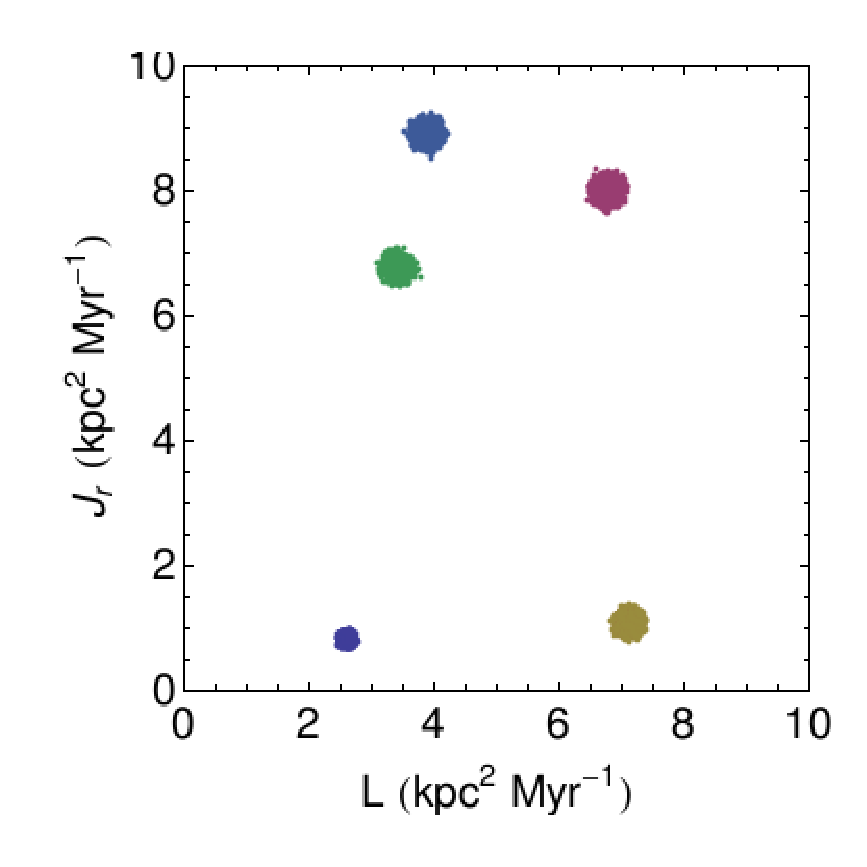
\includegraphics[width=0.32\textwidth]{InitialActions} & 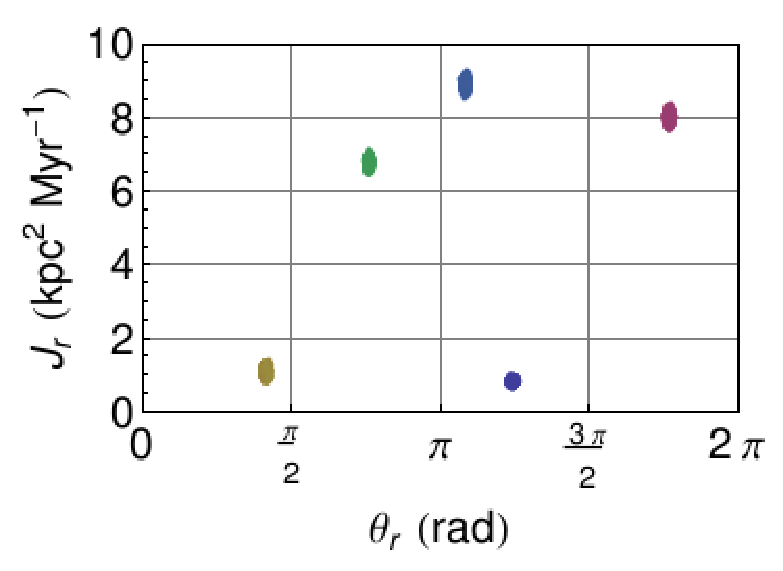
\includegraphics[width=0.32\textwidth]{InitialJrTheta5} & 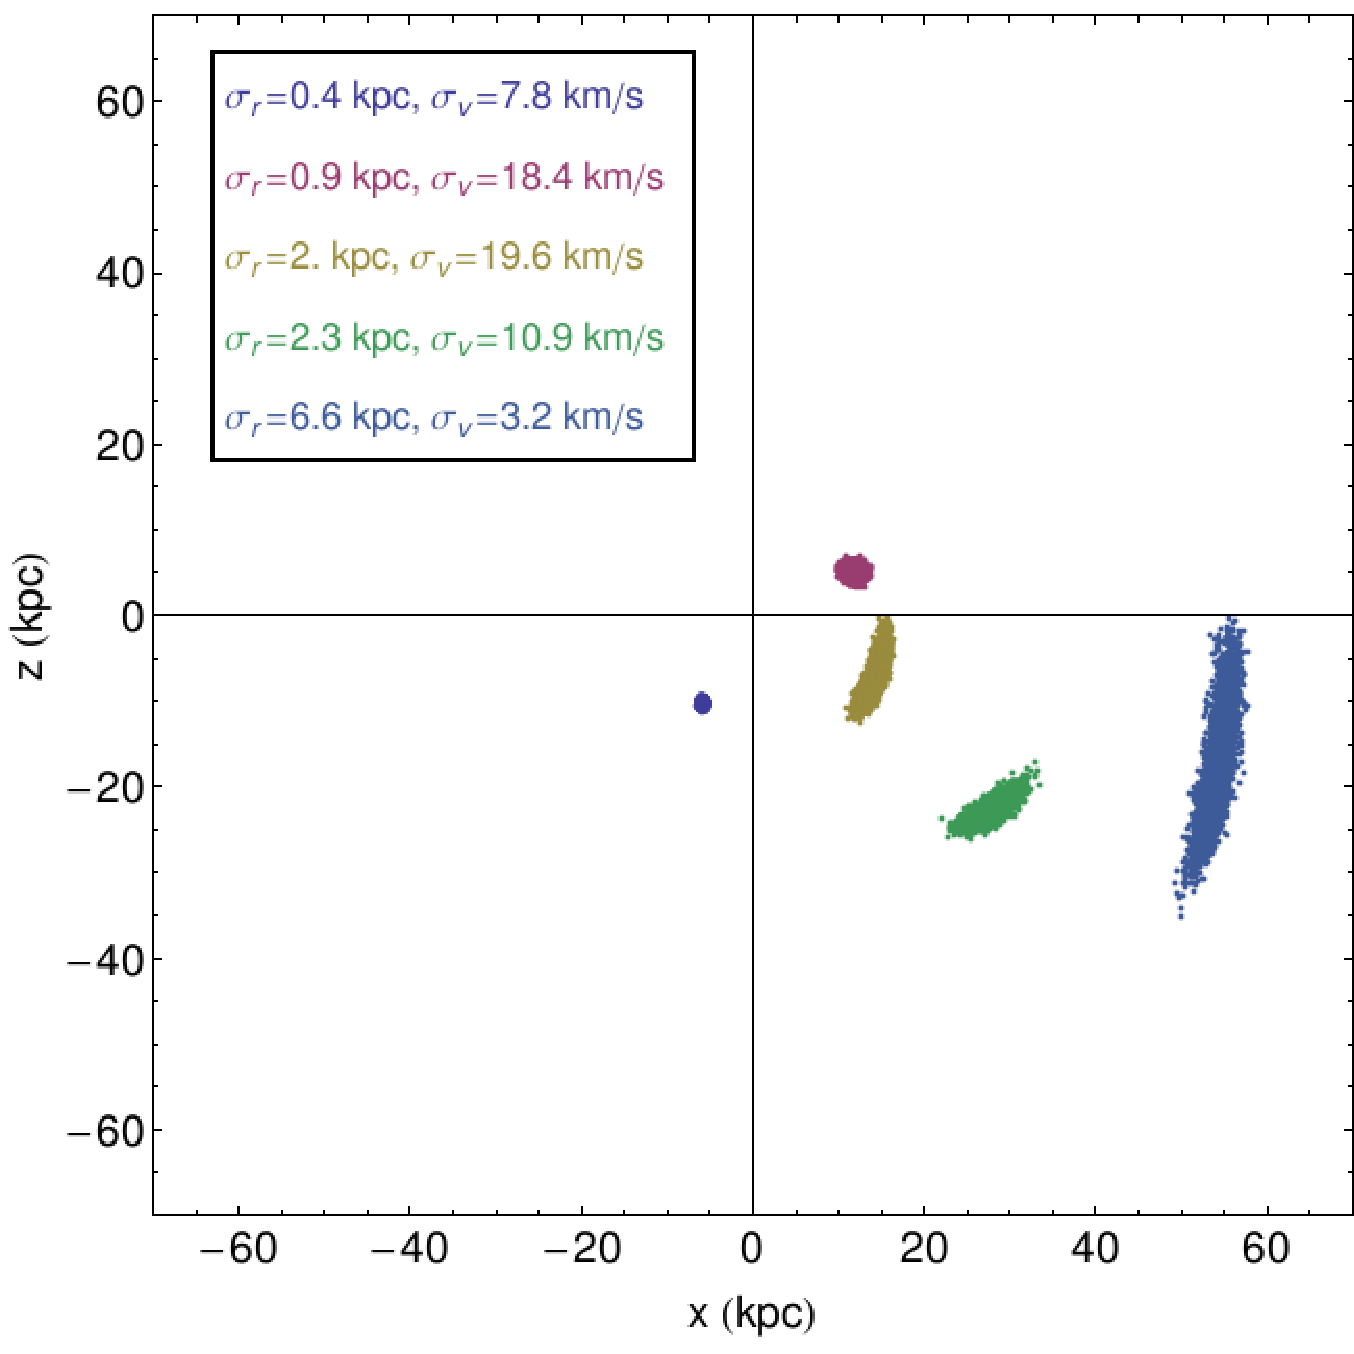
\includegraphics[width=0.32\textwidth]{InitXZ5}
\end{tabular}
\caption{Left: initial distribution of ``streams'' in action space. Center: initial distribution in a projection of angle-action space. Right: Projection of initial positions of the ``streams'' with measured one-dimensional dispersions in position ($\sigma_r$) and velocity ($\sigma_v$). }
\label{fig:initSetup}
\end{figure*}


To calculate the $(\mathbf{x},\mathbf{v})$ coordinates of the stream stars we must also specify the two remaining angles, those conjugate to $J_r$ and $L$. We use a two-step process to calculate the angles. First we generate ``initial'' angle values normally distributed around an initial point $\mathbf{\Theta}^0$ (chosen randomly between 0 and $2\pi$). The size of the normal distribution in each angle, as well as the action covariance matrix, are adjusted so that these initial clumps have physical sizes and velocity dispersions that resemble real dwarf galaxies. We take $\sigma_r$ in the range $\sim$0.1-10 kpc and $\sigma_v$ in the range $\sim$5-50 km/s. Because there is no self-gravity present in these models we can choose the spreads in action-angle variables to obtain any combination of $\sigma_r$ and $\sigma_v$, but large values of $\sigma_r$ tend to diagnose objects that are already partially disrupted, as shown when comparing the center and right panels of Figure \ref{fig:initSetup}.

Once we have a suitable set of initial angles, we evolve them forward in time for some duration $t$ using the frequencies $\mathbf{\Omega}(\mathbf{J})$, using the equations of motion
\begin{equation}
 \mathbf{\Theta} = \mathbf{\Theta}^{0} + \mathbf{\Omega}(\mathbf{J}) t.
\end{equation} 
We choose the evolution time $t$ to be different for each stream in the representation, so that some streams are still spatially coherent on the sky and others are well phase-mixed, as shown in the inset of Figure \ref{fig:streams}. For this work we choose $t$ randomly from 500 Myr to 5 Gyr for each stream. Finally we use the evolved values of the angles to calculate the $(\mathbf{x},\mathbf{v})$ coordinates of the stars in each stream. An example of the result for a system with 5 streams is shown in Figure \ref{fig:streams}.

\begin{figure}
 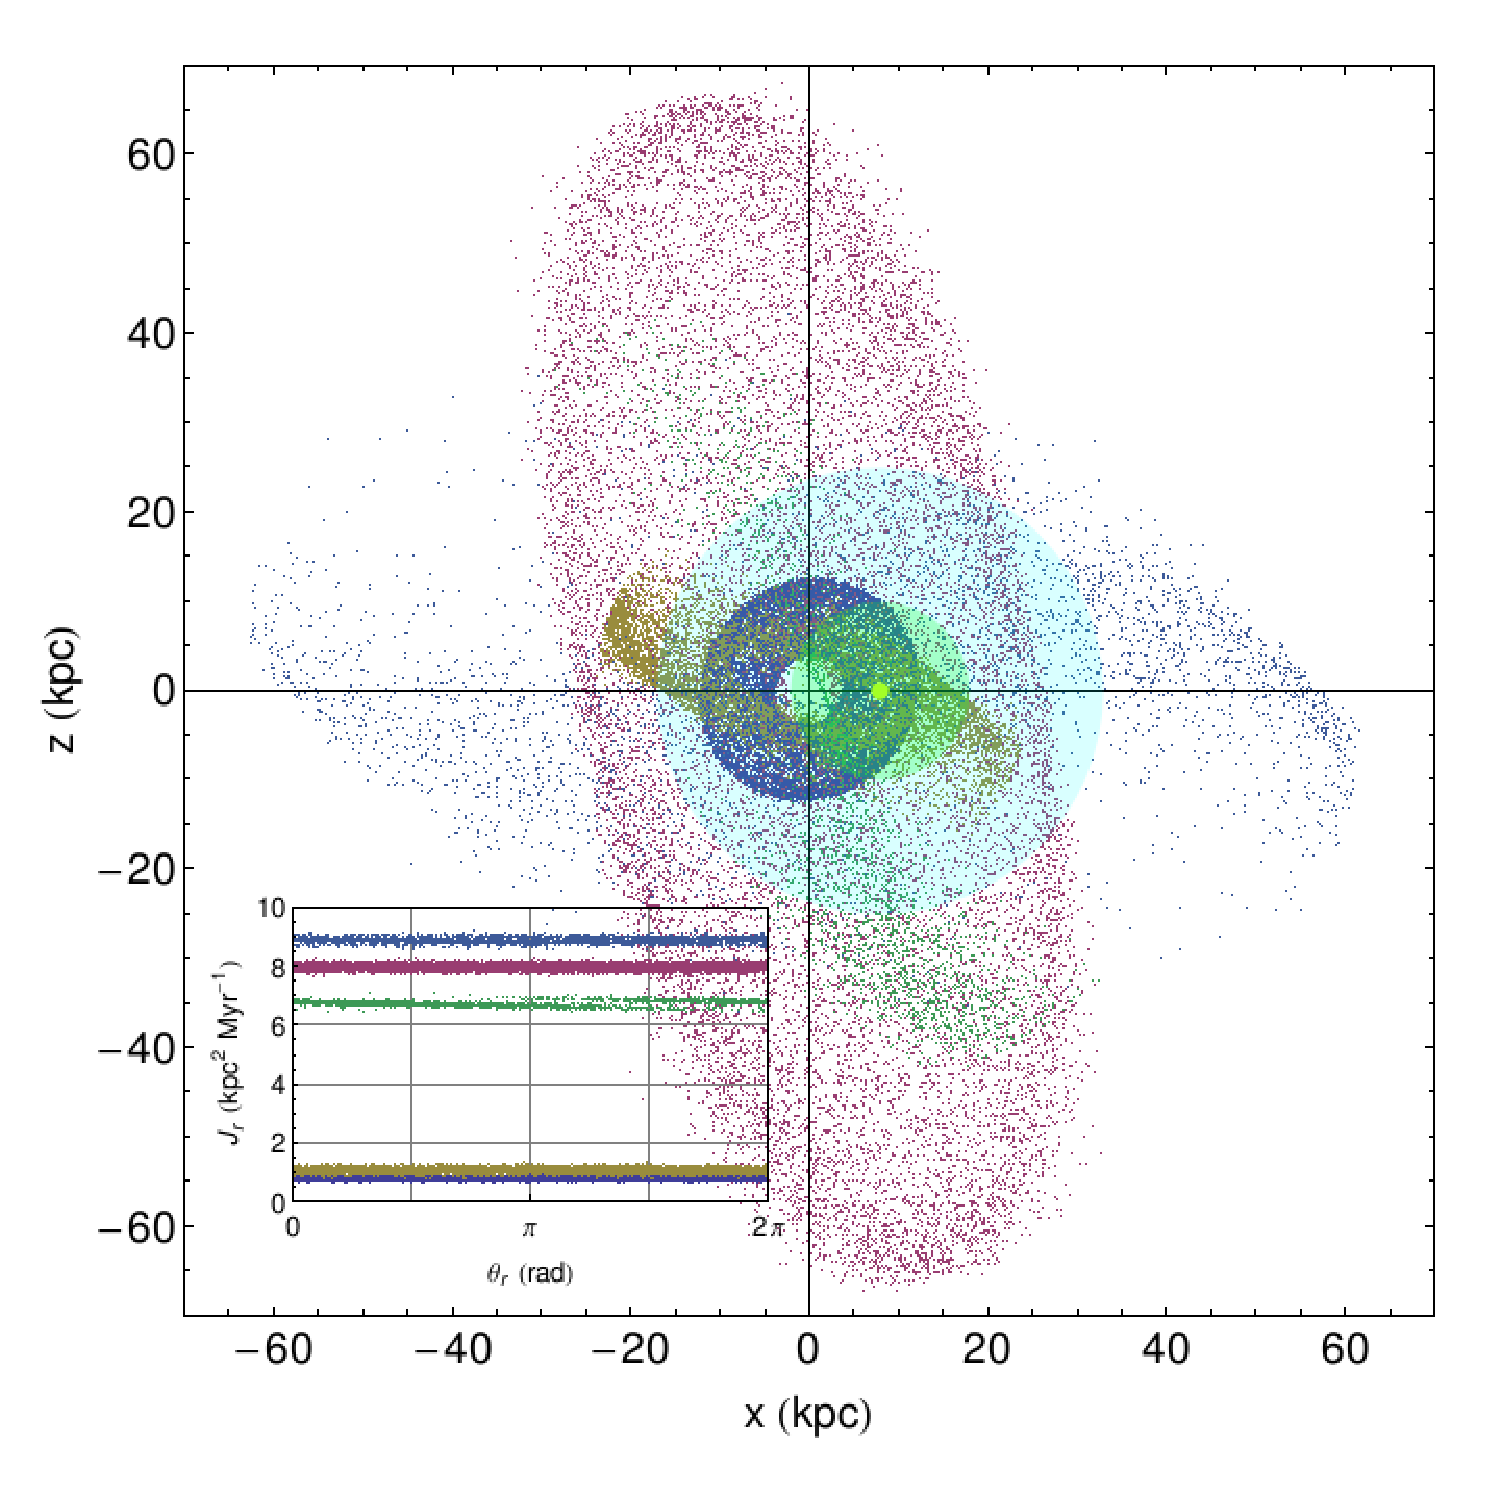
\includegraphics[width=0.45\textwidth]{FinalXZWithInset}
\caption{Projection in the $x$-$z$ plane of the positions of the stream stars after time-evolution. The yellow dot indicates the position of the Sun, which lies on the $x$ axis; the green and cyan circles indicate $\sub{d}{sun} < 10$ kpc and $\sub{d}{sun}<25$ kpc, respectively. Inset: result of the time-evolution in projected action-angle space. In this space the degree of phase-mixing of each stream is apparent: for example, the green stream is not completely phase-mixed since the ends of the distribution are still distinguishable, while the magenta stream forms a roughly solid band across the plot, indicating that the angle distribution is nearly uniform and the stream is well-mixed.}
\label{fig:streams}
\end{figure}

\subsection{Observables and noise convolution}

Once the above procedure is finished, we have $\mathbf{x}$ and $\mathbf{v}$ for each star in the set of streams. For the first set of tests described in this work, we simply use these as the input values to calculate the actions $\mathbf{I}_i(\mathbf{a})$, and hence the KL divergence, for various trial values of the potential parameters. These tests with ``perfect measurements'' are intended to identify any biases and degeneracies in the $\sub{D}{KL}$ surface, and give lower limits to the number of streams and number of stars per stream that are necessary to constrain the potential.

For a more realistic approach, we also add noise to the data based on the projected performance of upcoming astrometric and/or spectroscopic surveys. In this work we consider two cases: one in which the data come from the Gaia survey\footnote{\url{http://www.rssd.esa.int/index.php?page=Science_Performance&project=GAIA}}, and one in which the Gaia astrometry is supplemented by improved radial velocity measurements from one of two similar ground-based spectroscopic surveys (GBSS): WEAVE\footnote{\url{http://www.ing.iac.es/weave/}} (planned for the northern hemisphere) and 4MOST\footnote{\url{www.4most.eu}} (planned for the southern hemisphere). 

To simulate observational errors we start by calculating the observables $\mathbf{\varpi}$: parallax, proper motions, line-of-sight velocity (RV), and sky positions.  Then the expected error on each observable is determined based on the error models for Gaia and/or the GBSS (available from the project websites). To calculate the errors it is necessary to assign an absolute magnitude and spectral class to each star in the stream; we consider two simple cases rather than attempting to model a full stellar population. The first case assumes all the stars are red KIII giants with $M_V = 1$; the second assumes they are all main-sequence turnoff (MSTO) stars with $M_V = 4.5$. 

Once the errors have been calculated, each observable for each star is drawn from a one-dimensional Gaussian distribution centered on the true value with the width of the error. We assume that the errors on the observables are uncorrelated.  Then two data-quality cuts are made on the convolved observables to select all the stars with relative parallax error of less than 20\% and absolute line-of-sight velocity error less than 10 km \unit{s}{-1}. The distance errors dominate the error on all the coordinates; the RVs are the second most important source of error. We choose the parallax error cutoff to reflect the projected end-of-mission accuracy of the \emph{photometric} parallaxes from Gaia, and the RV error cutoff so that the actions recalculated with the noisy positions and the correct potential parameters are visibly clustered in $J_r-L$ space. This cutoff easily includes all stars observed by either GBSS, both of which project RV errors less than 2 km/s.

Finally, the cleaned set of observables are converted back into ``noisy'' 6D positions $(\tilde{\mathbf{x}}_i,\tilde{\mathbf{v}}_i)$. 

\subsection{Computation of the KL divergence}
We calculate the KL divergence $\sub{D}{KL}$ for a grid of different trial values of the potential parameters $\mathbf{a}$. The best-fit values, denoted $\mathbf{a}_*$, are the ones with the largest value of $\sub{D}{KL}$. Ideally we should find that $\mathbf{a}_* = \sub{\mathbf{a}}{true}$, but beyond this we want to examine how the contours of $\sub{D}{KL}$ behave: whether they lead clearly to a maximum at $\mathbf{a}_*$, and how they respond as we change $N_s$ or $N_*$. 

In the case of perfect measurements, the KLD is defined by Equation \eqref{eq:KLD_perfect}.  For noisy measurements, the actions themselves are now ``observations'' of the underlying distribution of the observables $\mathbf{\varpi}$, since they are computed from the observed values $(\tilde{\mathbf{x}}_i,\tilde{\mathbf{v}}_i)$ instead of the true values $(\mathbf{x}, \mathbf{v}$, so we write instead
\begin{equation}
\sub{D}{KL} \equiv \sum_i^{N_*} \log \frac{\tilde{O}[\tilde{\mathbf{I}}_i(\mathbf{a})|\mathbf{a}]}{\tilde{T}[\tilde{\mathbf{I}}_i(\mathbf{a})|\mathbf{a}]}.
\end{equation} 

To calculate $\sub{D}{KL}$ we therefore have to solve two technical problems. The first is how to infer $\tilde{O}$ from the discrete set of points $\tilde{\mathbf{I}}_i$. For this example we take a simple approach and use a $k$-nearest-neighbors density estimator, defined in $d$ dimensions as
\begin{equation}
 \tilde{O}(\tilde{\mathbf{I}}_i) = \frac{k \Gamma\left(d/2 + 1\right)}{N_* \pi^{d/2} r_{k,i}^d},
\end{equation} 
where $r_{k,i}$ is the distance to the $\super{k}{th}$ nearest neighbor of the $\super{i}{th}$ action tuple $\tilde{\mathbf{I}}_i$. Because all the actions have the same units, we can use the Euclidean distance function to calculate $r_{k,i}$. In two dimensions this expression is simply
\begin{equation}
 \tilde{O}(\tilde{J}_{r,i},\tilde{L}_i) = \frac{ k }{N_* \pi r_{k,i}^2}.
\end{equation}
We chose this strategy for inferring $\tilde{O}$ because it is simple, well-understood, and most importantly scale-free: the smoothing is controlled by the number of nearest neighbors $k$, which selects the smoothing length adaptively as a function of the density. An adaptive density estimator is crucial for computing the KLD: an estimator with a set smoothing length will automatically place an upper limit on the clustering in the distribution because any structures smaller than the smoothing scale will be lost. Additionally, streams will likely span a fairly wide range of sizes in their action-space distribution: objects from globular clusters ($10^6 M_\odot$) to the Magellanic Clouds ($10^{10} M_\odot$) are seen interacting with the Milky Way. Using an adaptive estimator avoids prioritizing streams with a particular progenitor mass (and hence action-space size). 

The second technical challenge in calculating the KLD is to establish a method for determining $\tilde{T}$ from the $\tilde{\mathbf{I}}_i$. A logical choice for $\tilde{T}$ would be the maximum-entropy distribution, a Gaussian with the same mean and standard deviation as $\tilde{O}$:
\begin{equation}
 T[\tilde{\mathbf{I}}_i(\mathbf{a})|\mathbf{a}] \equiv \frac{1}{\sqrt{(2 \pi)^k \det \mathbf{V}}} e^{-(\mathbf{I}-\mathbf{\mu})^T \mathbf{V}^{-1} (\mathbf{I}-\mathbf{\mu})/2},
\end{equation} 
where $\mathbf{\mu}$ are the means of the observed actions (first moment) and $\mathbf{V}$ is the covariance matrix (second moments). This choice guarantees that $\tilde{T}$ will be at least as smooth as $\tilde{O}$, but poses a technical problem that makes it very hard to use. As seen in Figure \ref{fig:actionClustering}, changing $\mathbf{a}$ away from the true values does not symmetrically broaden the density peaks associated with the streams. Instead it produces long tails to one side or the other of the distribution, sometimes with secondary peaks at the end of the tail (examples can be seen at large $J_r$ in both panels of the figure). The secondary peaks are a result of pile-ups (caustics) at the turning points of the stream orbits. These long tails tend to inflate the value of $\sub{D}{KL}$: they contain a relatively small number of stars compared to the total, so $\mathbf{\mu}$ and $\mathbf{V}$ are not changed too much, but they extend $\tilde{O}$ out to many times the width ($\sqrt{\det \mathbf{V}}$) of $\tilde{T}$, which drops off exponentially. Thus the few stars with the largest $\tilde{\mathbf{I}}$ can dominate the value of $\sub{D}{KL}$ for this choice of $\tilde{T}$, drowning out the true maximum not because $\tilde{O}$ is peaked, but because $\tilde{T}$ is very small (Figure \ref{fig:KLDGaussianSmooth}).

\begin{figure*}
 \begin{tabular}{cc}
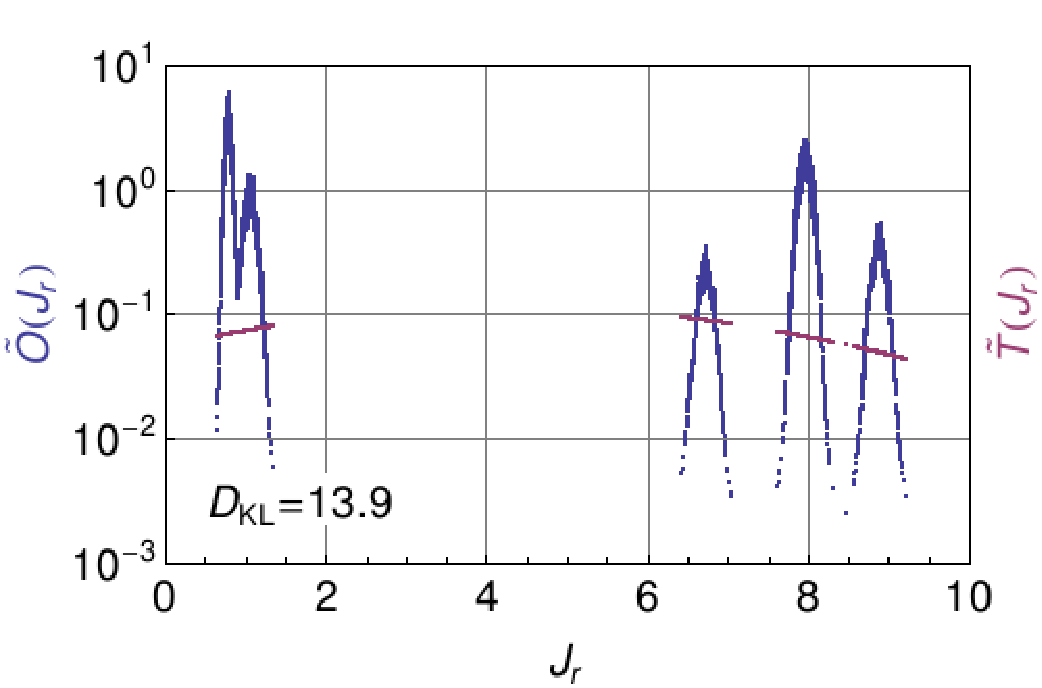
\includegraphics[width=0.45\textwidth]{KLDGaussianRight} & 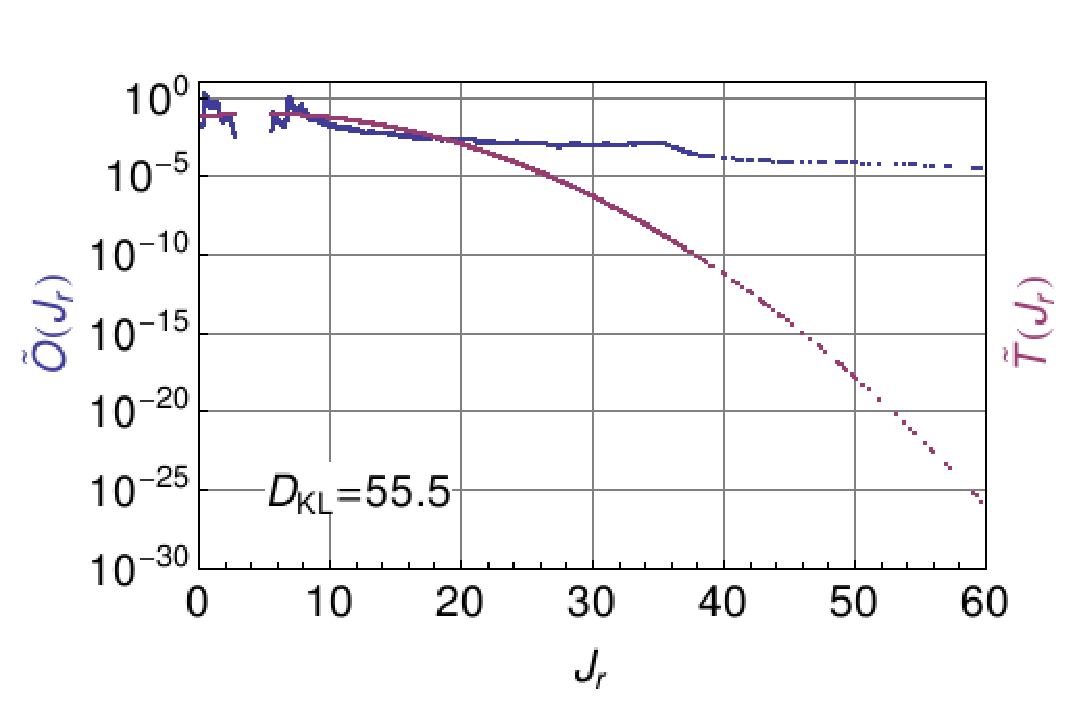
\includegraphics[width=0.45\textwidth]{KLDGaussianWrong}
\end{tabular}
\caption{With the correct potential parameters ($M=2.7\times10^12 M_\odot$, $b=8.0$ kpc), using a Gaussian asthe comparison distribution is well-behaved (left). However with slightly wrong parameters ($M=2.5\times10^12 M_\odot$, $b=9.5$ kpc), the long tails at high $J_r$ inflate the value of $\sub{D}{KL}$ thanks to the extremely small values of $\tilde{T}$ (right).}
\label{fig:KLDGaussianSmooth}
\end{figure*}


To solve this problem we use a different strategy for obtaining $\tilde{T}$ that exploits the multidimensionality of the system and the fact that manipulating $\mathbf{a}$ changes $J_r$ but not $L$ for this potential. We consider the action space $\tilde{\mathbf{I}}$ to be two-dimensional with coordinates $(J_r, L)$, and construct $\tilde{O}$ in two dimensions from this set of coordinates. Then we retain the $J_r$ value in each pair and shuffle all the $L$ values, smoothing out the distribution in the dimension that is insensitive to $\mathbf{a}$ as shown in Figure \ref{fig:shuffL}. The trial distribution $\tilde{T}$ is then obtained from the shuffled points in the same way as $\tilde{O}$. The loss of information in one of the two dimensions again guarantees that $\tilde{T}$ will be less peaked than $\tilde{O}$, just as in the maximum-entropy distribution, but this method does not suffer from the same range problems since the ranges of the two distributions are identical by construction.

\begin{figure*}
 \begin{tabular}{cc}
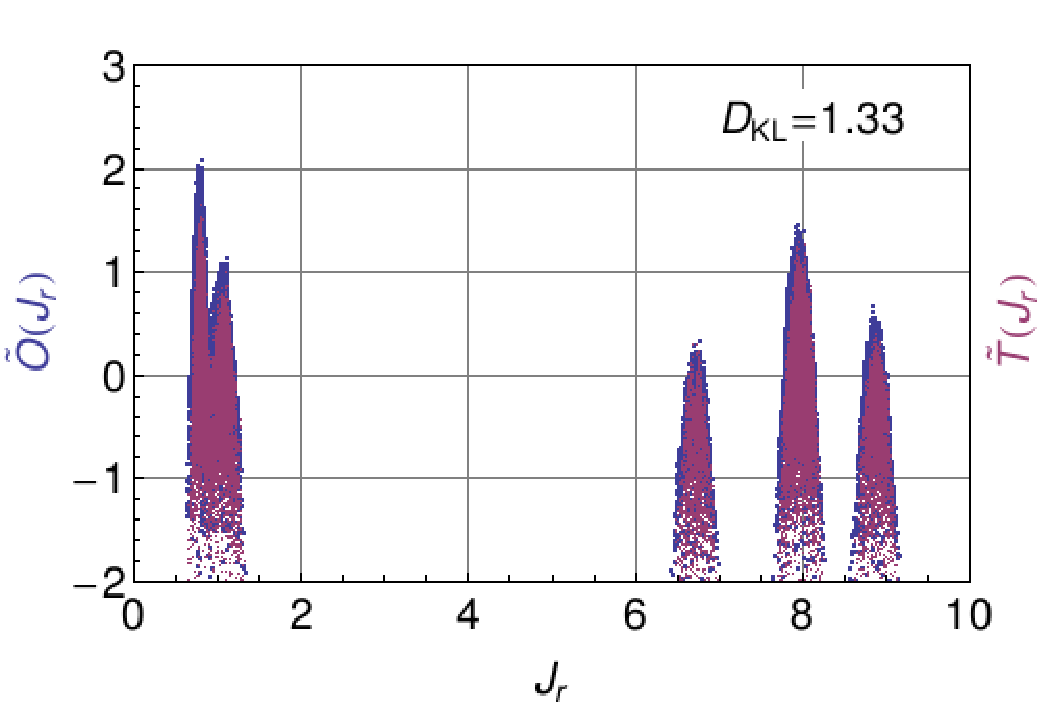
\includegraphics[width=0.45\textwidth]{KLDShuffleRight} & 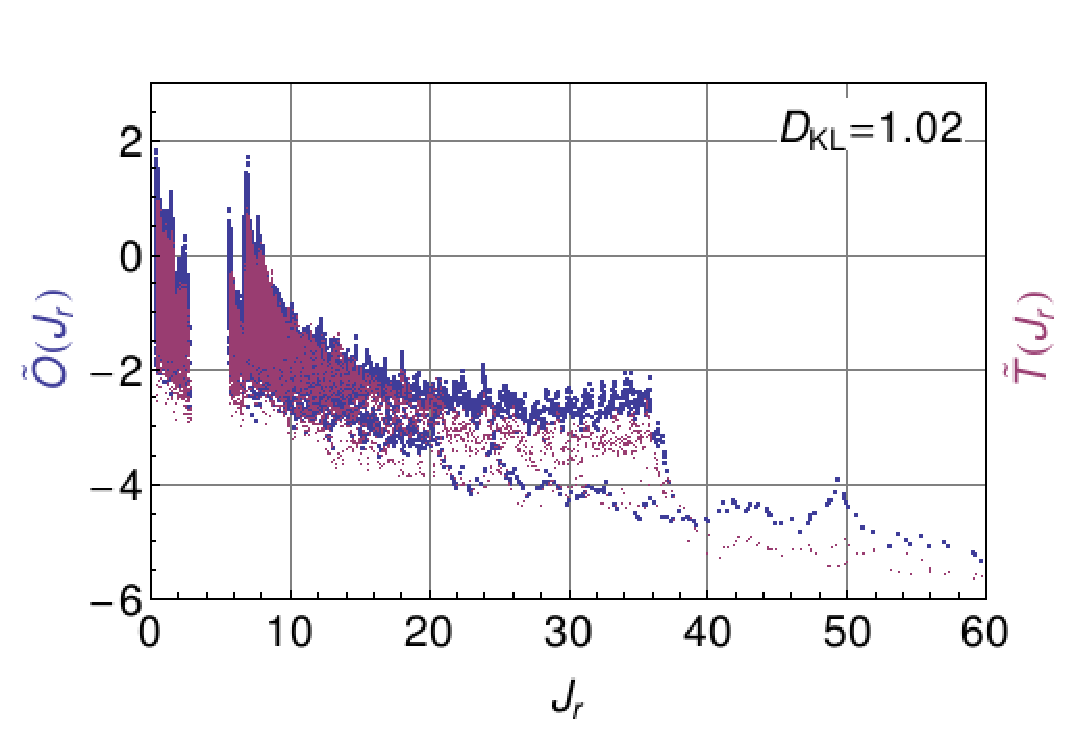
\includegraphics[width=0.45\textwidth]{KLDShuffleWrong}
\end{tabular}
\caption{Using the multidimensional shuffle method, the value of $\sub{D}{KL}$ for the correct potential parameters  (left) is still larger than for incorrect ones (right), but long tails at large $J_r$ no longer artificially inflate the value of $\sub{D}{KL}$. The values of the potential parameters in these plots are the same as in Figure \ref{fig:KLDGaussianSmooth}}
\label{fig:shuffL}
\end{figure*}

\section{Results with perfect measurements}

Before adding the step of convolving the star coordinates with observational errors, we first tested that the method recovered the input values of the potential parameters and examined the relative behavior of the error contours as a function of the number of stars or streams in the dataset. These results can be taken as lower bounds on the number of streams and stars per stream needed for the technique to work, since observational errors will reduce the amount of clustering even with the correct potential parameters.

The effect of changing the number of streams is shown in Figure \ref{fig:HowManyStreams}. To create these sets of contours, $N$ streams with random center-of-mass orbits were produced via the method described in Section \ref{sec:process}. The streams contain an average of 1000 stars each. 

\begin{figure*}
 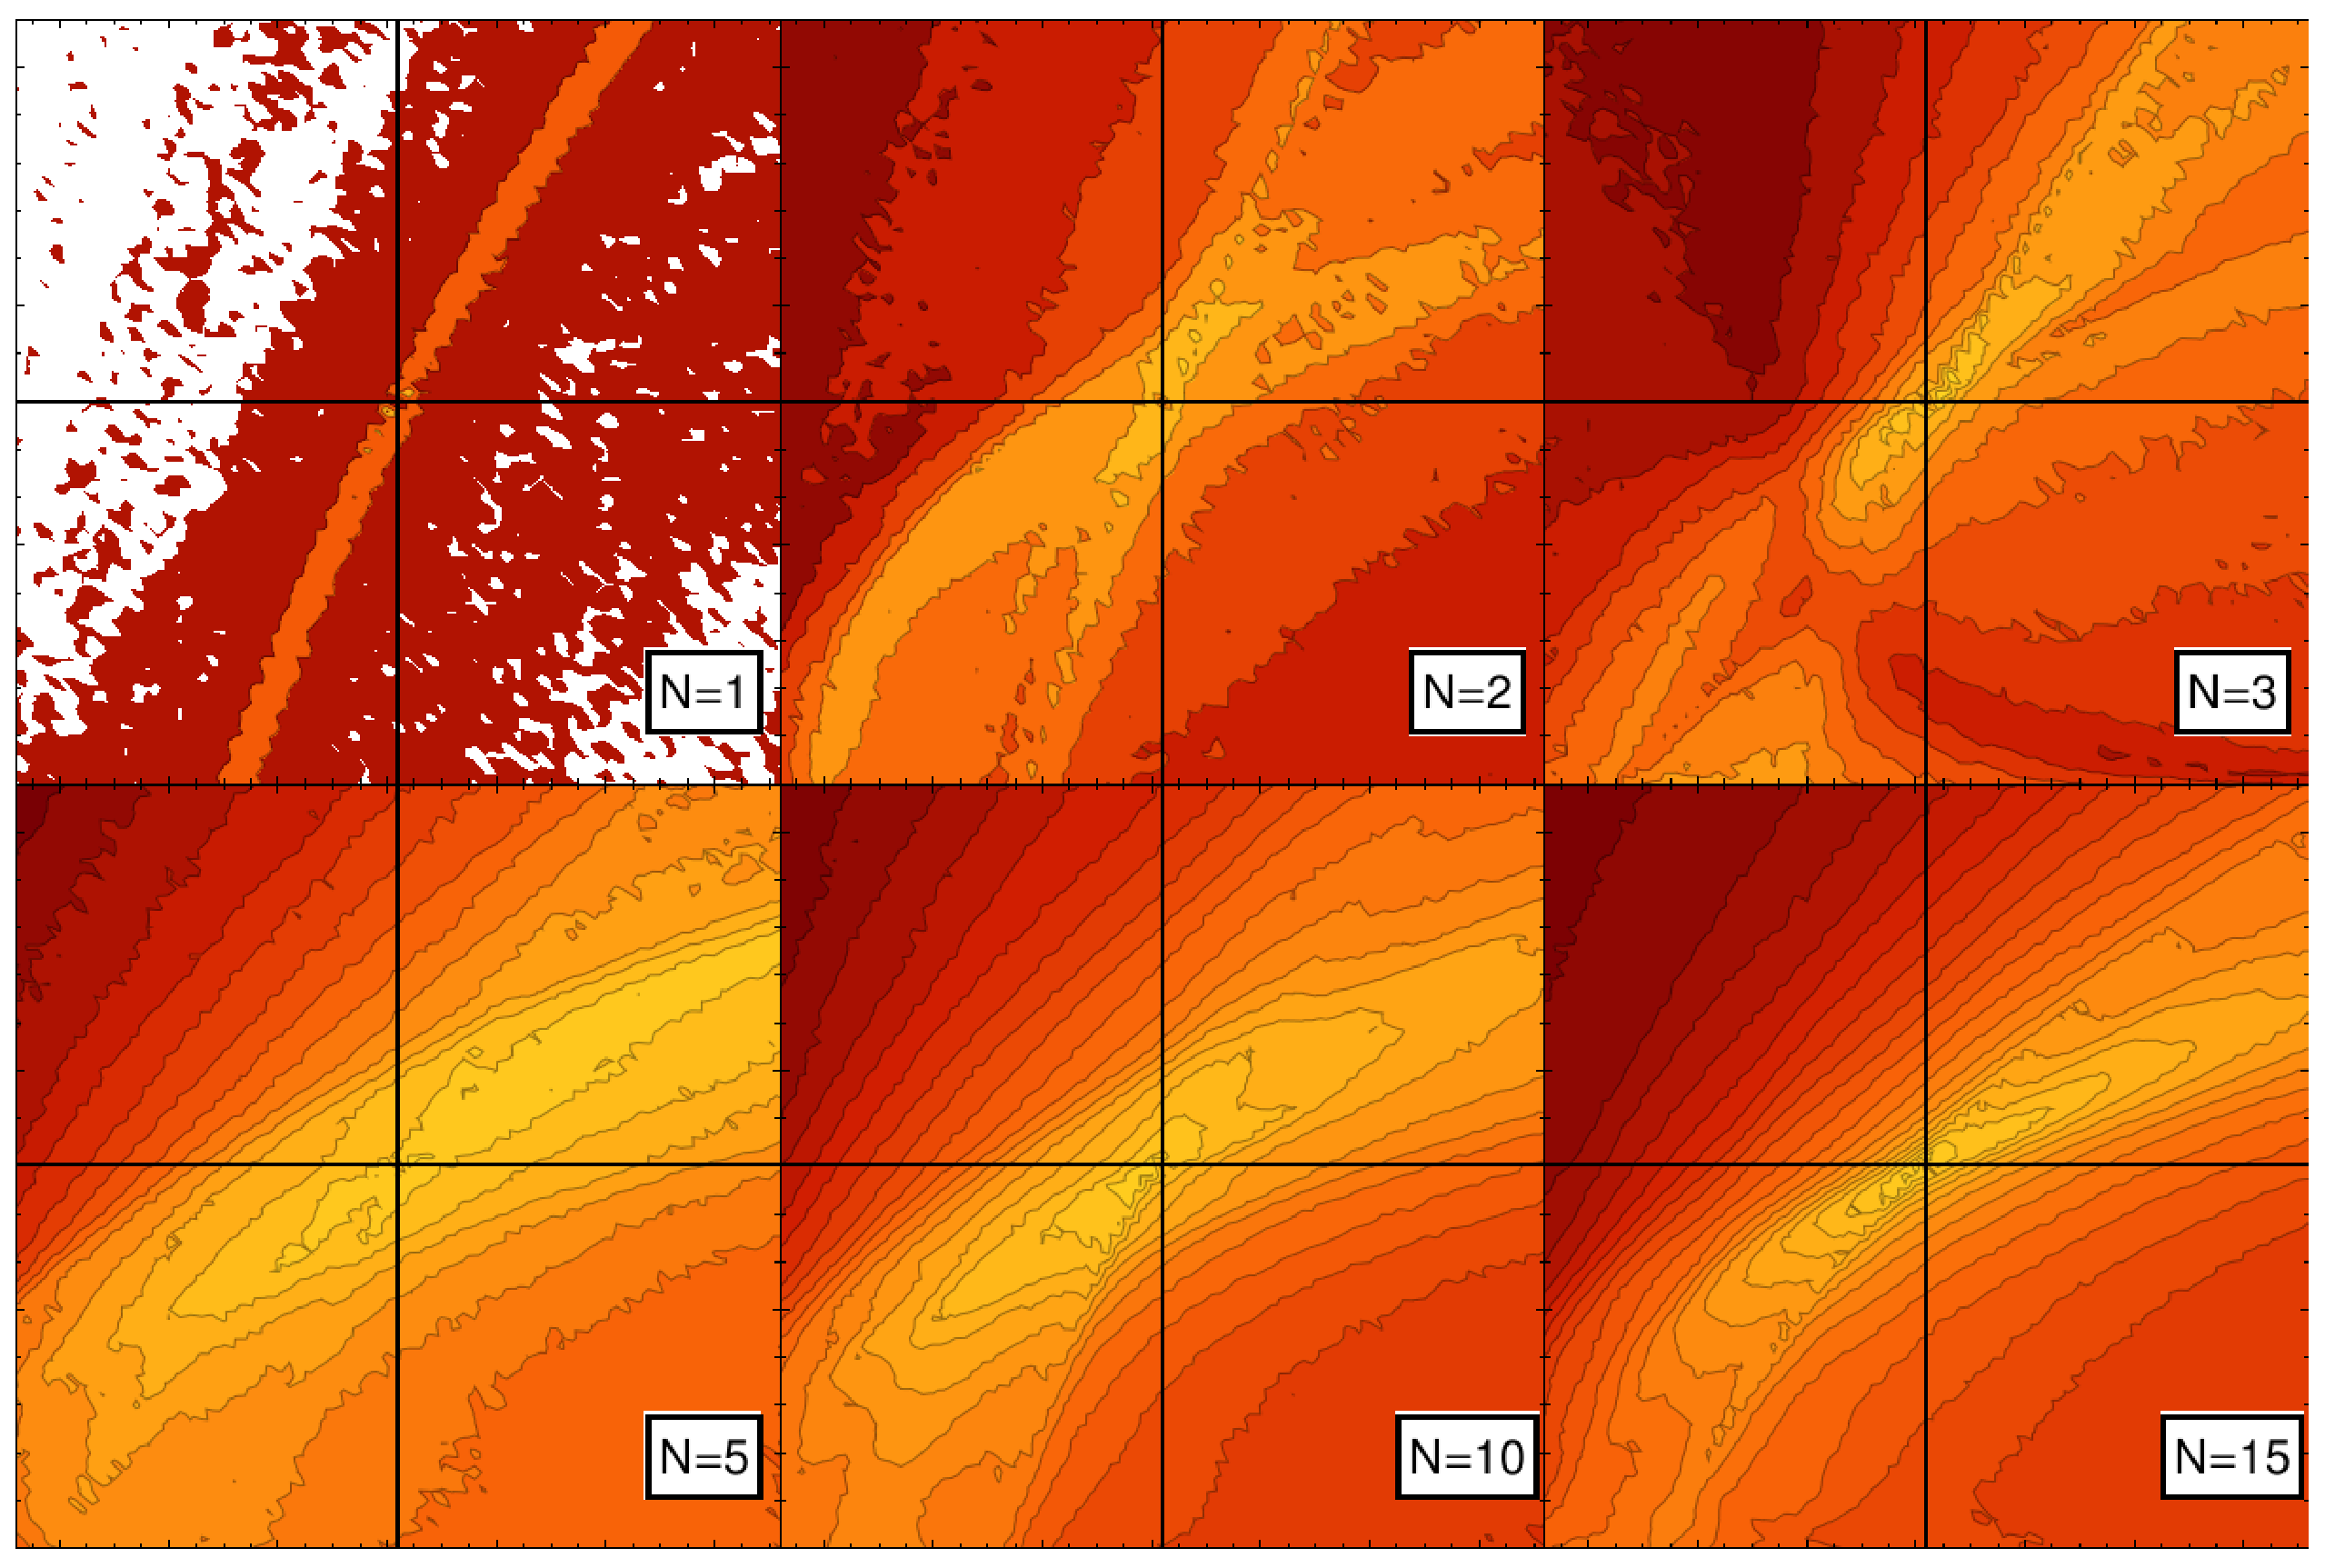
\includegraphics[width=0.95\textwidth]{HowManyStreams}
\caption{Contours of $\sub{D}{KL}$ for various numbers of streams $N$. The contour colors are the same in all the plots; the contours indicate intervals of 0.1 in $\sub{D}{KL}$ and range from 0 (reddest) to 2.6 (yellowest). In each panel, the $x$ axis spans a range of $M$ values from $1.2$ to $4.3 \times 10^{12}\ M_\odot$; the $y$ axis spans a range of $b$ values from 0 to 16 kpc. The black lines cross at the input values of $M = 2.7 \times 10^{12}\ M_\odot$ and $b = 8.0$ kpc.}
\label{fig:HowManyStreams}
\end{figure*}

It is evident that with only one stream (upper left corner), the enclosed-mass degeneracy between the two parameters cannot be broken.  With only 2 or 3 streams (top row), the ability to break this degeneracy and identify the best-fit parameters is sensitive to the particular orbits of the individual streams, so the contours look quite different from one panel to the next. Adding still more streams (bottom row), we find that the shape of the contours starts to regularize, the contours narrow around $\mathbf{a}_*$ and the contrast between the best-fit values and the rest of the parameter space improves. In all the panels except $N=1$, the best-fit $\mathbf{a}_*$ agree with the input $\sub{\mathbf{a}}{true}$.


Figure \ref{fig:HowManyStars} shows the effect of changing the number of stars per stream. Based on the results in Figure \ref{fig:HowManyStreams} all these trials were made with 5 streams, enough that the contours are not sensitive to individual stream details. The same set of 5 randomly generated streams was resampled with different numbers of stars $N$.

\begin{figure*}
 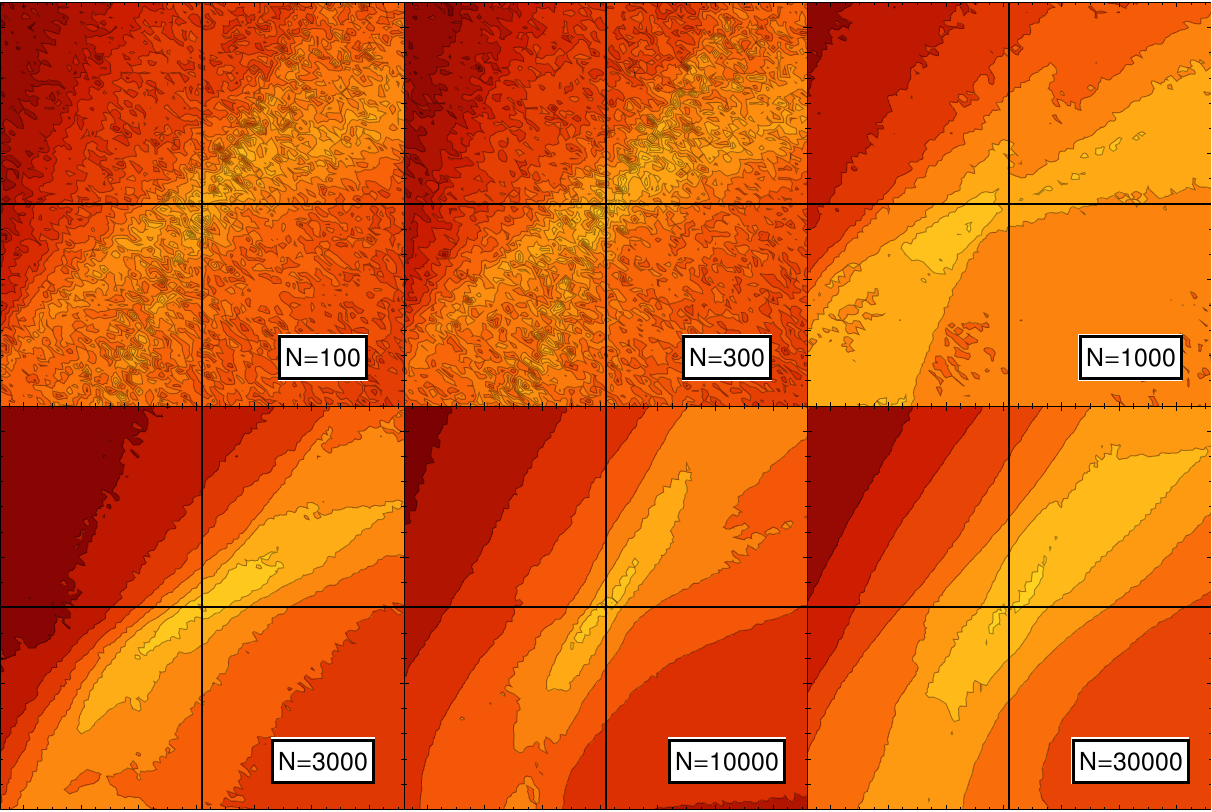
\includegraphics[width=0.95\textwidth]{HowManyStars}
\caption{Contours of $\sub{D}{KL}$ for various numbers $N$ of stars per stream. Again the contour colors are the same in all the plots but the contour interval in this case is 0.2. The contours range from 0 (reddest) to 3.4 (yellowest). The $x$ and $y$ axis ranges, and the black lines, are the same as in Figure \ref{fig:HowManyStreams}.}
\label{fig:HowManyStars}
\end{figure*}

At very low numbers of stars per stream, less than about 1000 (top left and top center), the underlying structure of the contours can be made out but the $\sub{D}{KL}$ surface is quite noisy. The noise level depends partially on the choice of $k$ in the density estimator; here we used $k=10$ which yields about 30 independent density samples per stream of 300 stars. With such a low $k$ the individual density estimates are fairly noisy as well. As the number of stars per stream increases, however, the noise level relative to the surface height decreases drastically. As the noise drops, the height and steepness of the best-fit peak also increases.

As expected, adding either more streams to the sample or more stars to the streams will improve the ability of this technique to constrain the potential parameters. Increasing the number of streams is necessary to break degeneracies in the parameters, while adding more stars refines the parameter constraints. Because of their degeneracy-breaking power the first priority should be to get as many streams as possible with some threshold number of stars per stream (here the threshold appears to be about 1000, but will also depend on observational errors). This is especially important because more realistic potential models will have many more than just 2 parameters and a much more complex set of degeneracies. So while technically two streams with a fortunate combination of orbits are enough to break the $M$-$b$ degeneracy in this simple example, in practice one or more additional streams will be needed for every new degeneracy among parameters.


\section{Results with observational errors} 

We also tested the performance of our method when star positions and velocities were convolved with observational errors. As summarized in Section \ref{sec:process}, we consider 4 basic cases: red giants and MSTO stars observed with Gaia only or with GBSS follow-up. Each test started with the same random sample of 10 streams with an average of 5000 stars per stream, for a total of 50000 ``true'' positions and velocities $(\mathbf{x}_i,\mathbf{v}_i)$. After error convolution we selected stars using data-quality cuts in $\sigma_\pi/\tilde{\pi}$ and $\sigma_{v_r}$, leading to a different ``cleaned'' sample size for each combination of stellar magnitude and error model. These are summarized in Table \ref{tbl:cleanSampleSizes}. 

\begin{table}
\caption{Number of stars satisfying data quality cuts.}
 \begin{tabular}{ccc}
 Stellar magnitude & Gaia only & Gaia + GBSS \\
\hline
``Red giants'' ($M_V = 1$) & 7775 & 24259 \\
``MSTO'' ($M_V = 4.5$) & 81 & 4183 \\
\end{tabular}
\label{tbl:cleanSampleSizes}
\end{table}


The distance of stars in the sample from the Sun is the most important factor in determining how many stars make the cut since this determines their apparent magnitude, which is the primary input to the error models. Both Gaia and the ground-based spectroscopic surveys have a target minimum apparent magnitude of $V=20$; Gaia will obtain radial velocities for stars with $V<17$ only. Figure \ref{fig:distanceHistogram} shows a histogram of the distances to the stars in the sample, marked with the maximum distances associated with these criteria for the two different absolute magnitudes used in this work. The total number of stars to the left of each of these lines is the base sample size for a given survey since anything to the right will not be observed. It is evident from the figure and Table \ref{tbl:cleanSampleSizes} that Gaia radial velocities alone will not allow us to include stars as faint as $M_V=4.5$ usefully into streams, while following up with ground-based spectroscopy can add a significant number of stars at this magnitude to streams in this distance range, especially given the fact that we expect many more stars with $M_v=4.5$ than  $M_V=1$. 

\begin{figure}
 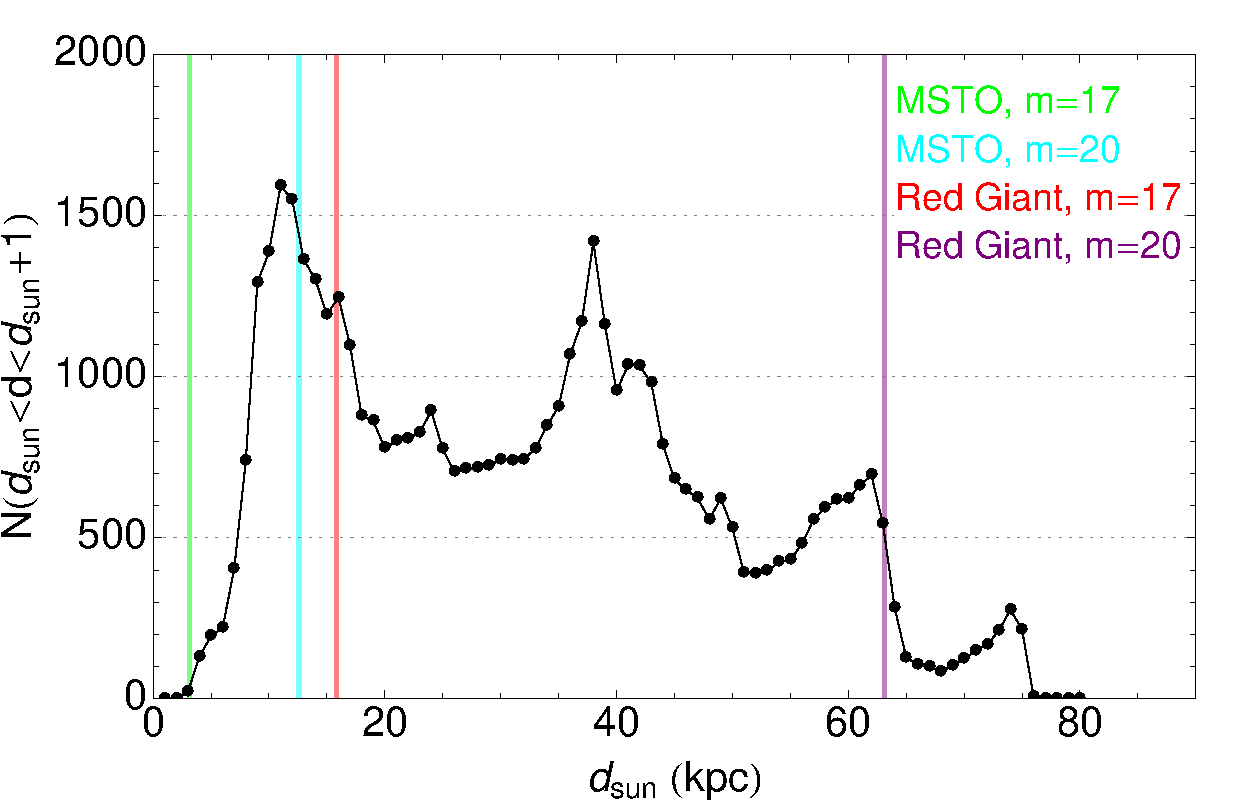
\includegraphics[width=0.45\textwidth]{dHist10}
\caption{Histogram of distances from stream stars to the Sun (located at (8,0,0) kpc) for the 10-stream sample to be convolved with observational errors. The colored lines indicate distances corresponding to the given absolute/apparent magnitude pairs.}
\label{fig:distanceHistogram}
\end{figure}



Figure \ref{fig:errorConvResults} shows the results for three of the four cases studied: we did not include the MSTO stars observed only with Gaia because so few had sufficiently small errors. Note that the case of MSTO stars with ground-based follow-up considers these stars alone, not added to the red giants; this is because we did not sample an appropriate ratio of the two populations so we cannot combine the two samples as would be done in principle. This means that not all the streams in the sample are included in this data set, explaining the slight bias and larger degree of degeneracy in this case compared to the other two. The improved RV coverage from ground-based spectroscopy significantly improves the ability to constrain the potential parameters relative to the Gaia-only case. 

\begin{figure*}
 \begin{tabular}{ccc}
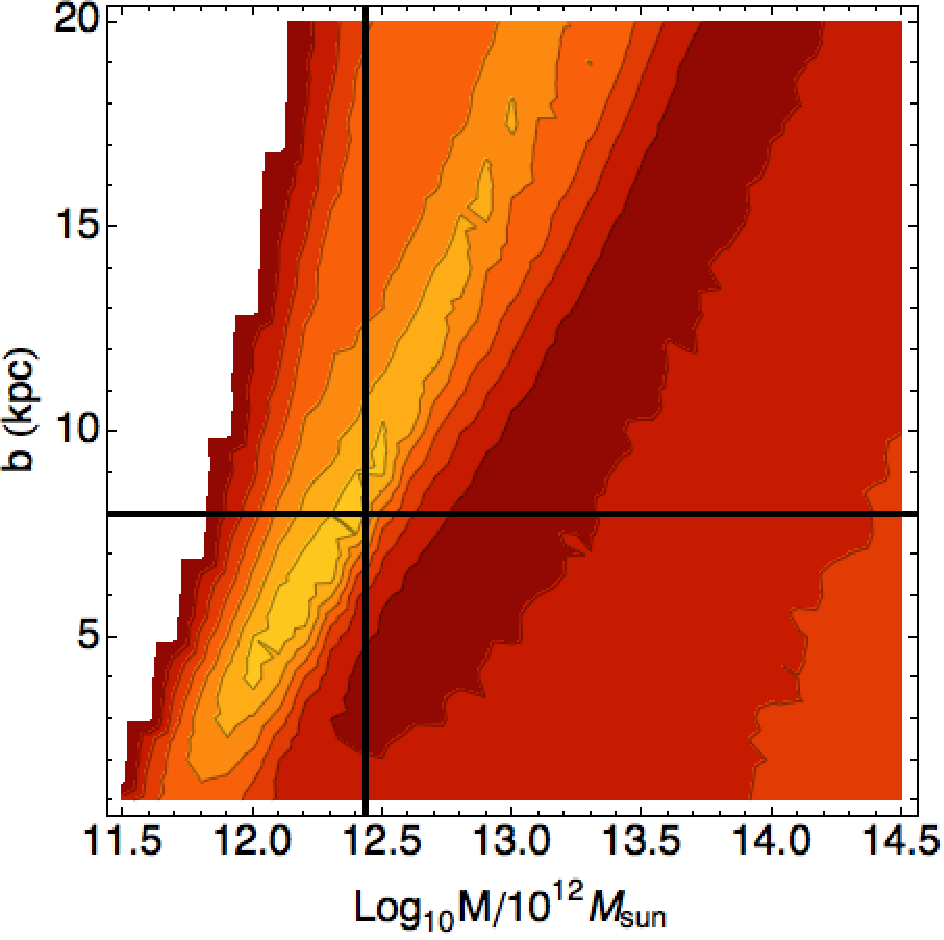
\includegraphics[width=0.31\textwidth]{KL10x5000LogM2D} & 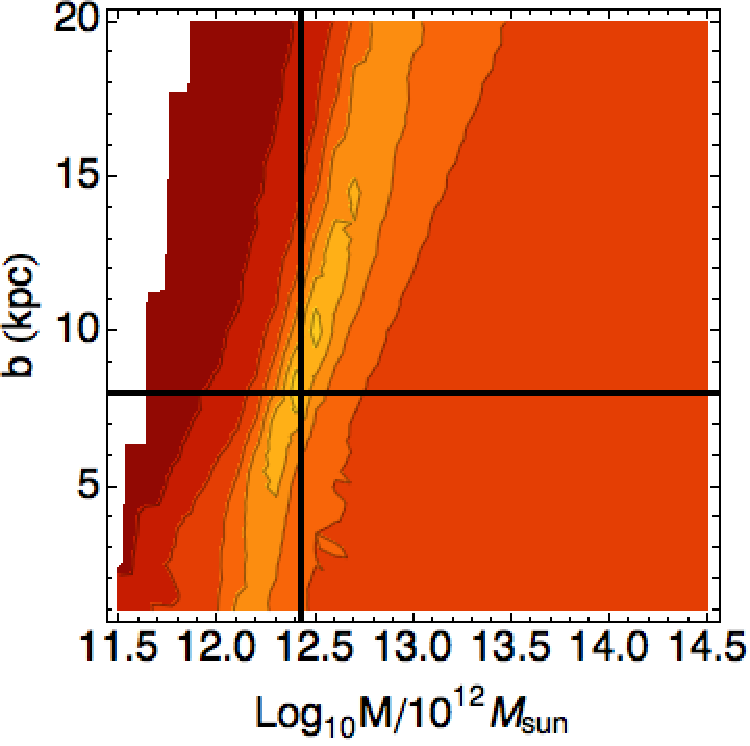
\includegraphics[width=0.31\textwidth]{KLDivRGs4MOSt} & 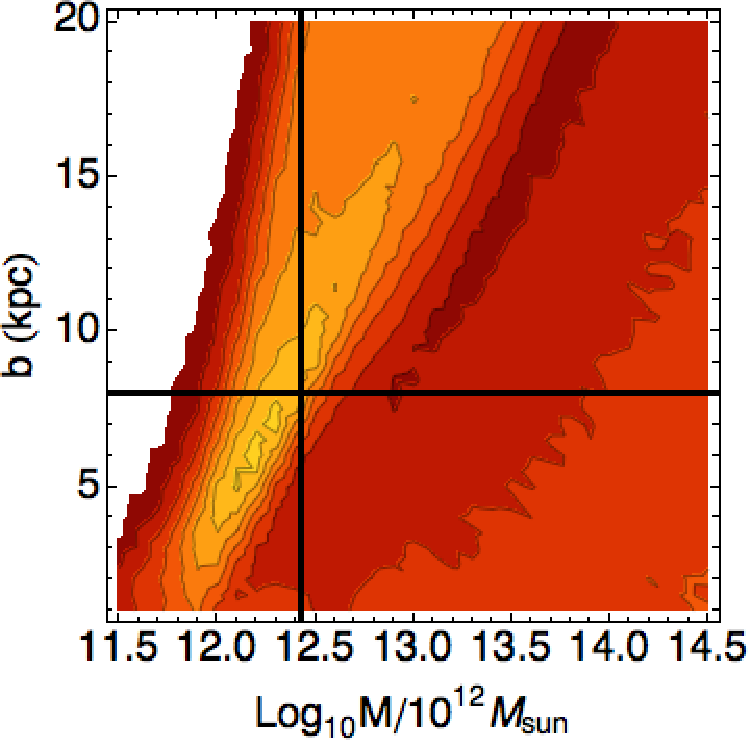
\includegraphics[width=0.31\textwidth]{KLDiv4MOST_MSTO}
\end{tabular}
\caption{Contours of $\sub{D}{KL}$ for Gaia only red giants (left), Gaia red giants with ground-based RVs (center), and Gaia MSTO stars with ground-based RVs (right). In all three plots the contours range from 0.05 to 0.75 in intervals of 0.1, except for the rightmost plot which goes up to 0.85. Note that the $M$ axis is now logarithmic.}
\label{fig:errorConvResults}
\end{figure*}


\section{Discussion \& Conclusions}

In this work we present a new method for constraining the Milky Way potential using the action space of stars in tidal streams. This method requires full six-dimensional phase-space information for all stars in the stream; such information will soon be available for large numbers of halo stars thanks to the Gaia satellite mission and associated ground-based follow-up spectroscopy. 

The method works on the principle that the actions of the stars in each stream are most tightly clustered when the potential used to calculate the actions is closest to the correct one. To measure the amount of clustering we use the Kullback-Liebler divergence. We show that maximizing the KLD recovers the input values for a simple example with several streams in the spherical isochrone potential. We further demonstrate that the method improves when more stars are observed per stream or when more streams are included; the former improves the steepness and contrast of the KLD surface around the maximum and the latter breaks degeneracies between parameters in the potential model. 

We explore the effect of observational errors by considering a case where 10 streams with 5000 stars each are identified; we find that Gaia observational errors are sufficient to apply this method for red giant stars ($M_V=1$). Supplementing Gaia astrometry with radial velocities for faint stars ($17<V<20$) from ground-based spectroscopic follow-up measurements greatly increases the number of stars (and therefore streams) available to this method, and allows the addition of MSTO stars ($M_V=4.5$) for nearby streams.


We have now laid the framework for exploring several important questions related to potential constraints in future work. First, the real Milky Way potential is not an exact copy of a parameterized model. We intend to explore the effect of imposing a fitted parameterization different from the input model: what parameters are recovered and what is their relation to the true potential? Second, some of the most interesting features of the halo concern its departures from spherical symmetry; we intend to expand the method to handle at least axisymmetric halos so that we can determine how well streams will constrain the flattening. Third, actions are superior to generic constants of the motion (such as energy) in part because they are adiabatically invariant; we intend to explore the effect of a slowly growing Milky Way in future work. Finally, this work considered only classes of stars, whereas in reality tidal streams have populations of stars. Using a more realistic model for the stream stars' types can produce better forecasts for the power of Gaia and other surveys to discover the shape of our Galaxy.

% 
% \subsection{Variations}
% 
%  Choose a different potential parameterization from the input one to calculate the ``observed'' actions and check how the shapes of the input and output potentials compare. If you fit the input potential at the points sampled with the output potential, you should get something close to the $\mathbf{a}_*$ obtained for the output potential.


%\section{Future ideas}
%\label{sec:future}
%\begin{itemize}
% \item more sophisticated potentials (closer to the realistic galaxy potential; this requires either Amina's Staeckel code or Binney's torus code, both of which I have access to)
%\item fitting streams from Aquarius using the above (like the ``wrong'' potential but more meaningful) 
%\item non-action spaces - poincare maps for example. Does the process still work if the actions$\leftrightarrow$poincare mapping is not one-to-one?
%\end{itemize}



%\bibliography{}

\end{document}